\documentclass{beamer}

\usetheme{metropolis}
\usepackage[french]{babel}
\usepackage[utf8]{inputenc}
\usepackage[T1]{fontenc}
\usepackage{graphicx}
\usepackage{tikz}
\newcommand{\roundimage}[2][2cm]{%
    \begin{tikzpicture}
    \clip[rounded corners=1cm] (0,0) rectangle (#1,#1);
    \node[anchor=south west, inner sep=0] at (0,0) {\includegraphics[width=#1]{#2}};
    \end{tikzpicture}%
}
\usepackage{pifont} % À mettre dans le préambule

% Icônes utiles
\newcommand{\question}{\ding{72}}   % ❓
\newcommand{\blocked}{\ding{55}}    % ��
\newcommand{\lock}{\ding{115}}      % ��
\newcommand{\target}{\ding{93}}     % ��


\setbeamertemplate{title page}{
    \vbox{}
    \vfill
    \begin{center}
    {\small % ⬅️ Réduction ici

    % Logos en haut
        \begin{minipage}{0.45\textwidth}
            \flushleft
            
\includegraphics[height=1.2cm]{logo}
        \end{minipage}%

        \vspace{0.5cm}

        {\usebeamerfont{title}\Huge \inserttitle\par}
        \vspace{0.3cm}
        {\usebeamerfont{subtitle}\Large \insertsubtitle\par}
        \vspace{1cm}
        {\usebeamerfont{institute}\normalsize \insertinstitute\par \usebeamerfont{date}\insertdate\par}

    } % fin du \small
    \end{center}
    \vfill
}

\setbeamertemplate{section in toc}[sections numbered]


% Informations
\title[Soutenance de Projet]{Soutenance de Projet}
\subtitle{SAE-821 Développement d’un
moteur de recommandations
respectueux de la vie privée}
\author{
    \textbf{Enzo Berge, Lois Hermelin}\\
    \textbf{Florian Audouard, Mattéo Pegliasco}
}
\institute{Université de Toulon, La Garde}
\date{2 Juin 2025}

\begin{document}

% Page de titre
\begin{frame}
    \titlepage
\end{frame}

% Sommaire
\begin{frame}
    \frametitle{Sommaire}
    \tableofcontents
\end{frame}

\section{Introduction}
\begin{frame}
    \frametitle{Introduction}
    \small
    Les moteurs de recommandation sont devenus omniprésents dans notre quotidien : sur les plateformes de streaming,
    les sites de e-commerce ou encore les réseaux sociaux. Leur but est de suggérer à l’utilisateur du contenu pertinent
    en se basant sur ses préférences, son historique de navigation ou les comportements d’utilisateurs similaires.

    Pour atteindre cette efficacité, ces systèmes s’appuient sur l’analyse de vastes quantités de données personnelles.
    Cette collecte, souvent invisible pour l’utilisateur, soulève de nombreuses préoccupations liées à la confidentialité
    et à la protection de la vie privée.

    Dans le cadre de ce projet, nous nous sommes donné pour objectif de concevoir un moteur de recommandations simple mais performant,
    capable de respecter les données personnelles des utilisateurs, en explorant des approches innovantes de préservation de la vie privée.
\end{frame}



% Problématique
\section{Problématique}
\begin{frame}
    \frametitle{Problématique}

    \small % Réduit la taille du texte

    \textbf{\question~Problème central :}
    \textit{Comment proposer des recommandations pertinentes sans compromettre la vie privée des utilisateurs ?}

    \vspace{0.2cm}
    \textbf{\blocked~Limites actuelles :}
    \begin{itemize}
        \item Solutions \textbf{centralisées} : profilage, tracking, fuites de données.
        \item Collecte massive de données personnelles.
    \end{itemize}

    \textbf{\lock~Deux approches de protection :}
    \begin{itemize}
        \item \textbf{Differential Privacy} : bruit pour anonymiser.
        \item \textbf{Cryptographie homomorphe} : calcul sur données chiffrées.
    \end{itemize}

    \textbf{\target~Objectif :}
    Développer un moteur de recommandation basé sur \texttt{MovieLens}, tout en garantissant la confidentialité.
\end{frame}

% User Story
\section{Conception UML}
\begin{frame}
    \frametitle{User Story}
    \small
    Le point de départ de notre projet repose sur une vision centrée utilisateur. La user story suivante résume notre objectif principal :
    \begin{block}
        \textit{« En tant qu’utilisateur, je veux recevoir des recommandations personnalisées sans que mes données personnelles soient stockées en ligne. »}\\
        \textit{« En tant qu’utilisateur, je veux pouvoir consulter mes avis sur les films que j’ai vus, sans que mes données personnelles soient stockées en ligne. »}\\
        \textit{« En tant qu’utilisateur, je veux pouvoir rechercher des films par titre/genres, sans que mes données personnelles soient stockées en ligne. »}
    \end{block}
    Cette phrase illustre une exigence fondamentale : proposer un service personnalisé tout en assurant une protection forte de la vie privée.
\end{frame}

\begin{frame}
    \frametitle{Diagramme de cas d'utilisation}
    \vspace{0.5cm}
    Ce qui nous donne le diagramme de cas d'utilisation suivant pour un utilisateur :
    \begin{center}
        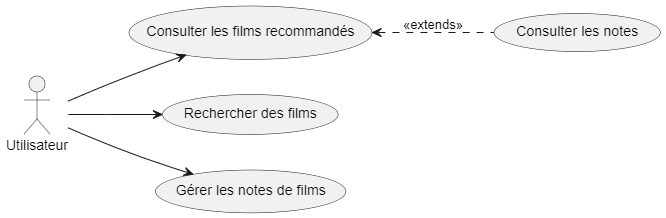
\includegraphics[width=0.75\textwidth]{uc_utilisateur.png}

        {\small Diagramme de cas d'utilisation de l'utilisateur}
    \end{center}
\end{frame}

\begin{frame}
    \frametitle{Diagramme de cas d'utilisation}
    \begin{center}
        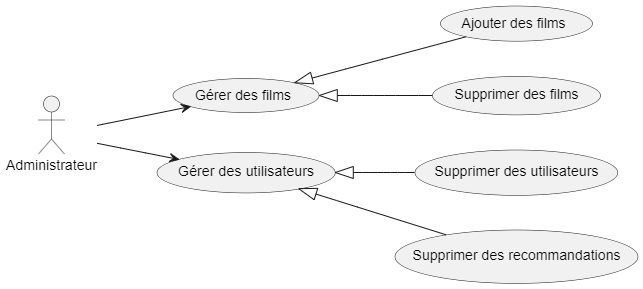
\includegraphics[width=0.75\textwidth]{admin.png}

        {\small Diagramme de cas d'utilisation de l'administrateur}
    \end{center}
\end{frame}


% Fonctionnalités - Vue générale
\section{Fonctionnalités}
\begin{frame}
    \frametitle{Fonctionnalités – Techniques}
    \small
    D’un point de vue technique, notre solution repose sur une architecture modulaire et des technologies robustes :

    \begin{itemize}
        \item \textbf{Filtrage collaboratif par SVD} : permet de réduire la dimensionnalité et d’identifier les similarités entre utilisateurs.
        \item \textbf{Bases de données} : utilisation de deux bases de données: PostgreSQL pour la manipulation et noSql pour l'accès rapide à la donnée
        \item \textbf{Differential Privacy} : ajout de bruit contrôlé aux données lors des échanges avec le serveur de recommandation et sélection biaisée pour la recommendation à froid.
        \item \textbf{Communication sécurisée par endpoints} : les échanges entre le back-end (serveur Quarkus) et le front-end sont encapsulés dans des requêtes REST sécurisées.
        \item \textbf{Interface avec React} : permet d’afficher dynamiquement les recommandations dans un environnement web léger.
    \end{itemize}

\end{frame}

% Architecture - Diagramme UML
\section{Architecture du système}
\begin{frame}
    \frametitle{Diagramme de classes}
    \vspace{0.5cm}
    \begin{figure}
        \centering
        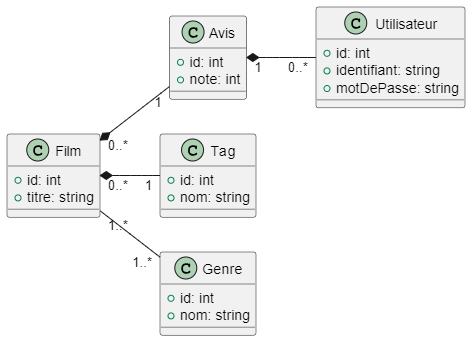
\includegraphics[width=0.75\textwidth]{classe.png}
        \caption{\small Diagramme de classes du système}
    \end{figure}
\end{frame}

\begin{frame}
    \frametitle{Diagramme de deploiement}
    \vspace{0.5cm}
    \begin{figure}
        \centering
        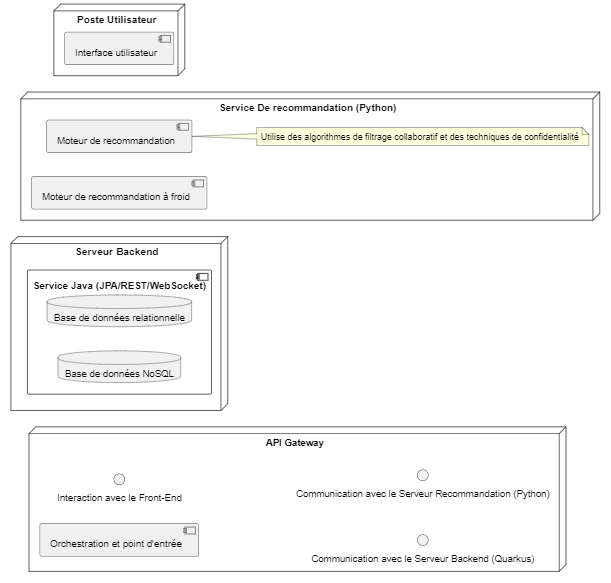
\includegraphics[width=0.60\textwidth]{deploiement.png}
        \caption{\small Diagramme de déploiement du système}
    \end{figure}
\end{frame}

% Choix et démarche
\section{Choix et démarche}
\begin{frame}
    \scriptsize
    \frametitle{Application Quarkus}
    \textbf{Organisation des classes: }conforme au modèle UML défini en amont, garantissant la cohérence entre conception et implémentation


    \textbf{Organisation des endpoints Quarkus:}
    \begin{itemize}
        \item \textbf{Controller :}  gère les requêtes HTTP et expose les endpoints REST.
        \item \textbf{Service : }contient la logique métier.
        \item \textbf{Repository: } s'occupe de l'accès aux données.
    \end{itemize}

    \textbf{Service d'importation de CSV: }automatisation de l'importation dans la base de données relationnelle et noSql
    \begin{itemize}
        \item Traitement par batchs (paquets) pour éviter les surcharges mémoire.
        \item Multi-threading en utilisant CompletableFuture pour accélérer l'import parallèle.
        \item Flush/Clear périodique de l’EntityManager pour libérer les ressources.
        \item Retry logique sur l’indexation Elasticsearch pour plus de robustesse.
    \end{itemize}
\end{frame}

\begin{frame}
    \scriptsize
    \frametitle{Application Quarkus(2)}
    \textbf{Authentification sécurisée: }vérification du mot de passe haché avec un salt : Le mot de passe est combiné à un salt unique, puis haché avec SHA-256 pour sécuriser les données stockées.

    \textbf{Intégration d’une base NoSQL avec Elasticsearch: } utilisé pour accélérer la recherche grâce à l’indexation des données (films, genres…), uniquement pour la consultation rapide, pas pour le traitement métier.

    \textbf{Quarkus : Serveur principal de l’application} est orchestré par un environnement docker compose
    \begin{itemize}
        \item \textbf{PostgreSQL :} base de données relationnelle principale.
        \item \textbf{Elasticsearch :} base NoSQL pour les recherches rapides via indexation.
        \item \textbf{API Python :} microservice dédié aux recommandations intelligentes.


    \end{itemize}



\end{frame}

\begin{frame}
    \scriptsize
    \frametitle{Système de recommandation}
    \vspace{0.3cm}
    {\large\textbf{Architecture générale}\\}
    \vspace{0.3cm}
    \textbf{Attributs nécessaire:}
    \begin{itemize}
        \item \textbf{Dataset}
        \item \textbf{Production (boolean)}
    \end{itemize}
    \vspace{0.3cm}
    \textbf{Méthodes nécessaire:}
    \begin{itemize}
        \item \textbf{Initialisation des données}
        \item \textbf{Entrainement du modèle}
        \item \textbf{Sauvegarde / Chargement du modèle}
        \item \textbf{Prédiction}
        \item \textbf{Précision}
    \end{itemize}
\end{frame}

\begin{frame}
    \scriptsize
    \frametitle{Système de recommandation}
    \vspace{0.3cm}
    {\large\textbf{Création des datasets}\\}
    \vspace{0.3cm}
    \begin{figure}
        \centering
        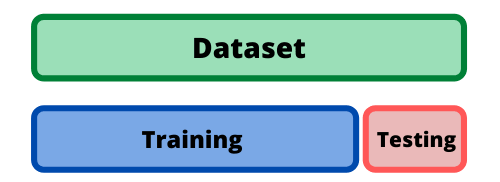
\includegraphics[width=0.60\textwidth]{trainset.png}
        \caption{Répartition des données en ensembles d'entraînement et de test}
    \end{figure}


\end{frame}

\begin{frame}
    \scriptsize
    \frametitle{Système de recommandation}
    \vspace{0.3cm}
    {\large\textbf{Métriques d’évaluation : précision et rappel}\\}
    \vspace{0.3cm}

    \begin{minipage}{0.3\linewidth}
        \centering
        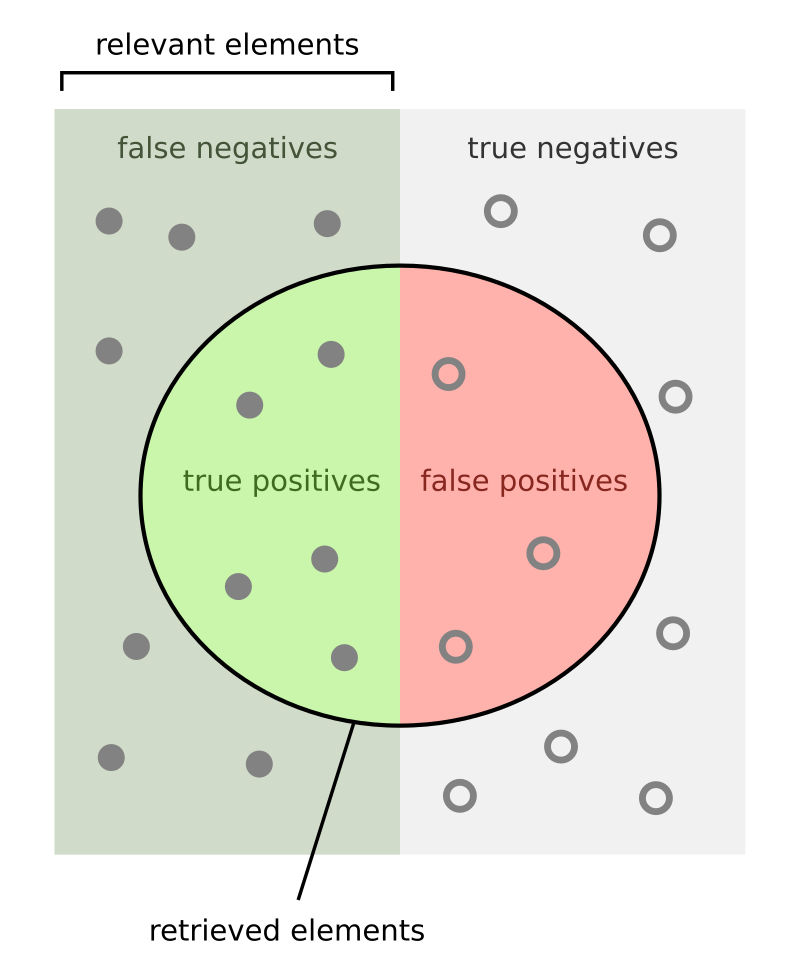
\includegraphics[width=\linewidth]{dataset_recall.png}
    \end{minipage}
    \hfill
    \begin{minipage}{0.65\linewidth}
        \centering
        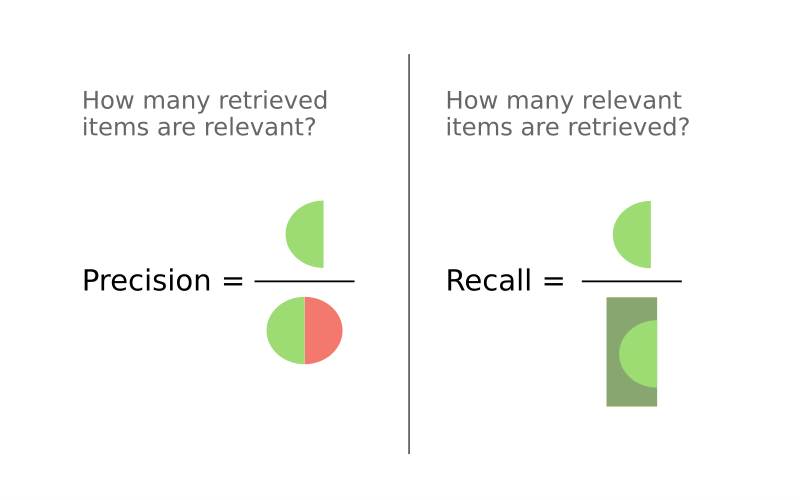
\includegraphics[width=\linewidth]{Precisionrecall.png}
    \end{minipage}


    \vspace{0.3cm}

\end{frame}
\begin{frame}
    \scriptsize
    \frametitle{Système de recommandation à chaud}
    \textbf{Contexte :} Utilisé lorsque l’utilisateur a un historique de notes ou d’interactions avec le système.

    \vspace{0.3cm}
    \textbf{Méthodes utilisées :}
    \begin{itemize}
        \item \textbf{Filtrage collaboratif} : basé sur les préférences d’utilisateurs similaires.
        \item \textbf{Matrix Factorization (SVD)} : extraction de facteurs latents pour modéliser les préférences.
    \end{itemize}

    \vspace{0.3cm}
    \textbf{Choix justifiés :}
    \begin{itemize}
        \item Fortes performances avec un dataset riche (MovieLens).
        \item Algorithmes bien adaptés à la personnalisation dynamique.
        \item Intégration fluide avec la Differential Privacy pour les échanges sécurisés.
    \end{itemize}
\end{frame}

\begin{frame}
        \scriptsize
        \frametitle{Differential Privacy}
        \textbf{Mise en place du bruit de Laplace :}
        Lors de des données des utilisateurs aud+ serveurs de recommendation, nous ajoutons un bruit de Laplace aux notes données par l'utilisateurs.
        
        \vspace{0.3cm}
        \textbf{Objectifs :}
        \begin{itemize}
            \item Brouiller les données des utilisateurs pour limiter l'extraction des informations personnelles depuis le systeme de recommendation.
            \item Assurer que les recommandations restent pertinentes malgré l'ajout de bruit.
            \item Conserver les données statistiques globales pour l'entraînement des modèles.
        \end{itemize}
    \end{frame}

    \begin{frame}
        \scriptsize
        \frametitle{Système de recommandation à froid}
        \textbf{Contexte :} Utilisé lorsque l’utilisateur n’a pas d’historique de notes ou pour les nouveaux utilisateurs.

        \vspace{0.3cm}
        \textbf{Méthodes utilisées : }
        \begin{itemize}
            \item \textbf{Les méthodes basées sur le contenu} : utilisent les similarités entre les items pour faire des recommendations.
            \item \textbf{Les approches hybrides} : combinent le filtrage collaboratif et le filtrage basé sur le contenu.
            \item \textbf{Les méthodes basées sur le clustering} : regroupent les utilisateurs ou les items selon leurs caractéristiques pour recommander des films.
    communes
        \end{itemize}

        \vspace{0.3cm}
        \textbf{Choix justifiés :}
        \begin{itemize}
            \item Complémentarité avec le système à chaud pour une couverture complète.
            \item Utilisation de DBSCAN pour gérer l'évolution de la base de données.
            \item Représenter la diversité des films présent dans la base de données.
        \end{itemize}
    \end{frame}

    \begin{frame}
        \scriptsize
        \frametitle{Differential Privacy (2)}
        \textbf{Mise en place du mécanisme exponentiel :}\\
        Ce mécanisme choisit des films en fonction de leur score de pertinence, tout en introduisant une part aléatoire contrôlée.

        \vspace{0.3cm}
        \textbf{Objectifs :}
        \begin{itemize}
            \item Protéger la vie privée des utilisateurs en rendant difficile l’inférence des notes globales attribuées aux films.
            \item Proposer des recommandations pertinentes selon certains critères, comme l’écart maximal de la note moyenne par rapport à 2.5.            
        \end{itemize}
    \end{frame}

% Déroulement du projet
\section{Déroulement du projet}
\begin{frame}
    \frametitle{Déroulement du projet}
    \scriptsize

    Le projet a été mené selon une méthodologie \textbf{agile} structurée en \textbf{sprints hebdomadaires}. Chaque lundi, une réunion de planification permettait de définir les tâches à réaliser, accompagnées d’un \textbf{chiffrage en points de charge}.
    \vspace{0.1cm}
    Un \textbf{rapport journalier textuel} était rédigé tout les jours pour assurer un suivi continu de l’avancement.

    \vspace{0.1cm}
    \textbf{Outils} :
    \begin{itemize}
        \item \textbf{Python} : langage principal pour le développement du moteur de recommandation
        \item \textbf{GitHub} : collaboration, versionnement, documentation
        \item \textbf{Quarkus} : architecture backend
        \item \textbf{React} : front-end pour la visualisation locale
    \end{itemize}
    Tous les éléments (code, docs, rapports) sont sur GitHub pour une architecture micro-service et une collaboration efficace.

\end{frame}


\section{Résultats}
\begin{frame}
    \frametitle{Résultats obtenus : SVD}
    \scriptsize
    \textbf{Notre système a permis d’atteindre plusieurs objectifs clés, tant sur le plan fonctionnel que technique :}

    \vspace{0.3cm}
    \begin{itemize}
        \item \textbf{Prototype opérationnel} : système complet de bout en bout avec SVD.
        \item \textbf{Qualité des recommandations} :
              \begin{itemize}
                  \item Précision : 72.2\% / 71.8\%
                  \item Rappel : 69.1\% / 68.6\%
              \end{itemize}
        \item \textbf{Respect de la vie privée} :
              \begin{itemize}
                  \item Échanges bruités par Differential Privacy
              \end{itemize}
        \item \textbf{Mesure des performances (temps)} :
              \begin{itemize}
                  \item Initialisation des données : 0.14 s
                  \item Entrainement du modèle: 0.72 s
                  \item Temps de réponse moyen : 0.03 s
              \end{itemize}
    \end{itemize}
\end{frame}

\begin{frame}
    \frametitle{Résultats obtenus : Deep Learning}
    \scriptsize
    \textbf{Notre système a permis d’atteindre plusieurs objectifs clés, tant sur le plan fonctionnel que technique :}

    \vspace{0.3cm}
    \begin{itemize}
        \item \textbf{Prototype opérationnel} : système complet de bout en bout avec un modèle d’apprentissage profond.
        \item \textbf{Qualité des recommandations} :
              \begin{itemize}
                  \item Précision : 72.6 \% / 71.3\%
                  \item Rappel : 69.3\% / 67.5\%
              \end{itemize}
        \item \textbf{Respect de la vie privée} :
              \begin{itemize}
                  \item Échanges bruités par Differential Privacy
              \end{itemize}
        \item \textbf{Mesure des performances (temps)} :
              \begin{itemize}
                  \item Initialisation des données : 0.08 s
                  \item Entrainement du modèle: 0.68 s
                  \item Temps de réponse moyen : 0.03 s
              \end{itemize}
    \end{itemize}
\end{frame}

\begin{frame}
    \frametitle{Résultats obtenus : Clustering non supervisé}
    \scriptsize
    \textbf{Nos Objectifs étant de favoriser la diversité tout en représentant les élèments de la base de données  :}
    (609 test réalisés avec une réduction à 150 dimensions et 20 films demandés et une meme seed aléatoirey)
    \vspace{0.3cm}
    \begin{itemize}
        \item \textbf{Qualité des recommandations} : (non bruité / bruité)

              \begin{itemize}
                  \item Diversité des genres : 60.9 \% / 60.4 \%
                  \item Sélections films peu noté moyennes : 23.5\% / 26.3\%
                  \item Couverture des recommendations: 23\% / 24.7\%
                  \item Nombre moyen de clusters : 8.87 / 8.8 (pour 10 clusters)
                  \item Ratio films par utilisateur : 2.57 / 2.63
              \end{itemize}
        \item \textbf{Mesure des performances (temps)} :
              \begin{itemize}
                  \item Initialisation des données :  0.02 s
                  \item Entrainement du modèle : 180 s
                  \item Temps de réponse moyen : 0.006 s
              \end{itemize}
    \end{itemize}
\end{frame}

% Perspectives
\section{Perspectives}
\begin{frame}
    \frametitle{Perspectives d'évolution}
    \small
    \begin{itemize}
        \item \textbf{Explorer d'autres approches de recommandation à froid} :
              améliorer la rapidité et la précision et explorer l'ajout de statistiques de données contextuelles pour la recommendation par clustering.

        \item \textbf{Repenser l'architecture microservices} :
              réduire les fortes dépendances entre les modules pour gagner en modularité, maintenabilité et résilience.

        \item \textbf{Automatiser l’initialisation des données} :
              remplacement des appels manuels aux endpoints par des scripts d’initialisation ou des pipelines de données.

        \item \textbf{Intégrer un modèle de langage (LLM)} :
              générer des recommandations contextuelles plus riches grâce à l’exploitation de texte ou de préférences complexes.

        \item \textbf{Améliorer l’interface utilisateur} :
              créer un front-end plus moderne, esthétique et responsive pour renforcer l’engagement utilisateur.
    \end{itemize}
\end{frame}



\begin{frame}[c]
    \centering
    
\includegraphics[width=0.4\textwidth]{logo.png}

    \vspace{1cm}
    {\Huge \textbf{Merci pour votre attention !}}

    \vspace{1.5cm}
    {\Large N'hésitez pas à poser vos questions !}
\end{frame}

\end{document}